%MIT OpenCourseWare: https://ocw.mit.edu
%RES.18-011 Algebra I Student Notes, Fall 2021
%License: Creative Commons BY-NC-SA 
%For information about citing these materials or our Terms of Use, visit: https://ocw.mit.edu/terms.

\section{Normal Subgroups and Quotient Groups}
\subsection{Review}
In the last lecture, we learned about the correspondence theorem. 

\begin{theorem}[Correspondence Theorem]
Where $f: G \rightarrow G'$ is a surjective\footnote{In fact, it is possible to slightly revise the statement of the theorem such that the surjective condition is no longer necessary.} homomorphism, and $K = \ker(f),$ there is a correspondence 
\[
\{\text{subgroups } H: K \subseteq H \subseteq G\} \leftrightsquigarrow \{\text{subgroups } H' : \{e_{G'}\} \subseteq H' \subseteq G'\}\},
\]

which states that subgroups of $G$ containing the kernel are in bijection with subgroups of $H'$ in the image of $f.$
\end{theorem}

The correspondence comes from taking 
\begin{align*}
H &\mapsto f(H) \subseteq G' \\
\{x \in G : f(x) \in H'\} = f^{-1}(H') &\mapsfrom H'
\end{align*}

From the point of view of understanding subgroups, the correspondence theorem allows us to understand a slice of $G.$ If $G$ is a complicated group with many surjective maps onto different groups $G',$ we can use the correspondence theorem multiple times to understand $G,$ and conversely, if $G'$ is a complicated group, we can use $G$ to study $G'.$ 

\begin{proof}
In order to show that this correspondence is a bijection, we check that these are inverses to each other. 
\begin{itemize}
    \item If $K \subseteq H \subseteq G,$ then we want to show that $f^{-1}(f(H)) = H.$ By definition, 
    \[ 
    f^{-1}(f(H)) = \{x \in G : f(x) = f(h), h \in H\}.
    \]
    By definition, $H \subseteq f^{-1}(f(H)).$ Also, if $x \in f^{-1}(f(H)),$ then $f(x) = f(h)$ for some $h \in H.$ This is true if and only if $x$ is in the coset $hK;$ in other words, $x = h\cdot k$ for some $k \in K.$ Since $K \subseteq H,$\footnote{The theorem is \emph{not} true if the kernel is not contained in $H$, so this fact must be used at some point.} $k \in H,$ and so $x = hk \in H.$ 
    \item The proof of the other direction is left as an exercise to the reader (it is very much the same idea).  
\end{itemize}
\end{proof}


\subsection{Normal Subgroups}

Recall the definition of a normal subgroup.
\begin{definition}
A subgroup $H \subseteq G$ is \textbf{normal} if $xHx^{-1}= H$ for all $x \in G.$
\end{definition}

The notation $H \leq G$ denotes that $H$ is a subgroup, not just a subset, of G. Now, the notation $H \trianglelefteq G$ will denote that $H$ is a \emph{normal} subgroup of $G.$\footnote{This notation will not necessarily be used consistently throughout this lecture/class, but it is used in the literature.}

\begin{example}[Kernel]
The kernel $\ker(f)$ is \emph{always} normal.
\end{example}

\begin{qq}
Given any normal subgroup $N \nsub G$, is there always a group homomorphism $f: G \rightarrow G'$ such that $N = \ker(f)$?

\textbf{Answer:} Yes!
\end{qq}

Let's look at a quick example first. 
\begin{example}[Integers modulo 2]
If $G = \ZZ$ and $H = 2\ZZ,$ the homomorphism is 
\begin{align*}
G &\xrightarrow{f} G' = \ZZ_2 \\
n &\mapsto n \mod 2.
\end{align*} 

The kernel of $f$ consists of the elements mapping to $0 \mod 2$; that is, even integers, which is precisely $2\ZZ.$ 
\end{example}

In the case when $N = \ker(f),$ the cosets\footnote{The left and right cosets are the same when $N$ is normal.} of $N$ are in correspondence with $\im(f),$ by the correspondence theorem. Since they are in bijective correspondence, the group structure on $\im(f)$ can be carried over to the set of cosets of $N.$

%** write out explicitly why the correspondence theorem gives us this!! im slightly confused

\begin{center}
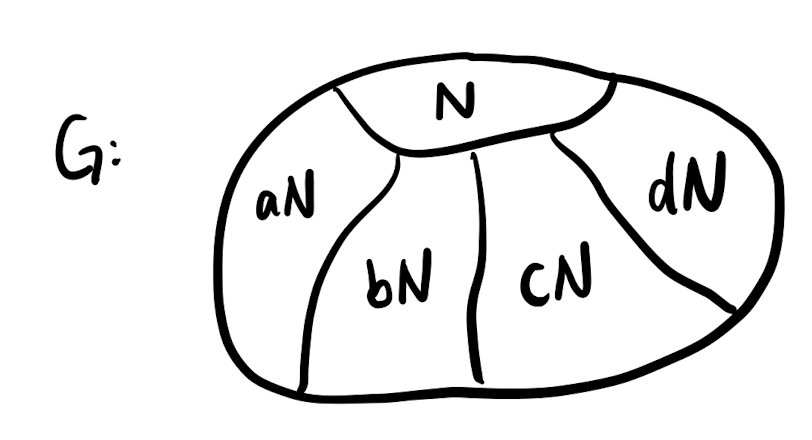
\includegraphics[width = 5cm]{Lecture Files and Images/lec6-3.png}
\end{center}

\subsection{Quotient Groups}

Now that we've defined cosets, we have the following question:
%\textbf{Guiding Question.} 

\begin{qq}
Can we directly define a group structure on the sets of cosets of $N$?
\end{qq}

If $C_1, C_2 \subseteq G$ are cosets, what should $C_1 \cdot C_2$ be? The most intuitive definition would be to take the set of products of each of the elements:

\begin{definition}\label{product of cosets is cosets}
Let the product structure on the cosets be defined as \[C_1 \cdot C_2 \coloneqq \{x \in G: x = y_1 \cdot y_2 ; y_1 \in C_1, y_2 \in C_2\},\]
the pairwise product.
\end{definition}
\begin{theorem}
If $C_1, C_2$ are cosets of a normal subgroup $N$, $C_1 \cdot C_2$ is also a coset of $N.$ 
\end{theorem}

It is \emph{crucial} that $N$ is normal! 
\begin{example}
Consider $H = \{e, y\} \subseteq G = S_3.$ Then $H$ is not a normal subgroup. Consider $xH = \{x, xy\}$. We have \[
xH \cdot xH = \{x^2, x^2y, xyx = y, xyxy = e\},
\]
which is \emph{not} a coset!
\end{example}

\begin{proof}
Let $C_1 = aN$ and $C_2 = bN.$

\begin{itemize}
    \item The inclusion $abN \subseteq C_1 \cdot C_2$ holds because $abn = (ae)(bn) \in C_1 \cdot C_2,$ since $ae \in C_1$ and $bn \in C_2.$ 
    
    \item Take $an_1 \cdot bn_2 \in C_1 \cdot C_2.$ Since $N$ is normal, $bN = Nb,$ so $n_1 \cdot b = b \cdot n_3$ for some $n_3 \in N.$ So 
    \[
    an_1 \cdot bn_2 = abn_3n_2 \in abN.
    \]
\end{itemize}

Then $C_1 \cdot C_2 = abN.$ 

\end{proof}

So it is only when $N$ is normal that we do in fact have a product structure on the set of cosets of $N$!
\begin{definition}\label{quotient group}
The \textbf{quotient group} $G/N$ is the set of cosets of a normal subgroup $N.$ The group structure is defined as\footnote{The notation $[x]$ refers to the equivalence class of $x$ under an equivalence relation; in this case, the equivalence relation is defined by the partition of $G$ into cosets.}
\begin{align*}
[C_1] \cdot [C_2] &\coloneqq [C_1 \cdot C_2] \\
[aN] \cdot [bN] &\coloneqq [abN].
\end{align*}
The right hand side is a coset because $N$ is a normal subgroup.\footnote{The product can be verified to be independent of the representatives $a$ and $b$ from the fact that $N$ is normal.} %\footnote{Did we prove that it is independent of the representatives $a$ and $b$?}
\end{definition}

\begin{theorem}\label{quotient group composition}
The following two statements are true about the quotient group:
\begin{enumerate}
    \item The composition law, as defined in Definition \ref{quotient group} \emph{does} define a group structure on $G/N$ (all the group axioms hold).
    \item There exists a surjective homomorphism 
    \begin{align*}
    \pi: G &\rightarrow G/N \\
    x &\mapsto [xN]
    \end{align*}
    such that $\ker(\pi) = N.$
\end{enumerate}
\end{theorem}

This is one of the most basic operations we can do on groups! 

\begin{proof}

First of all, let's show that $G/N$ is actually a group.
\begin{itemize}
    \item \textbf{Identity.} The identity is $[N] = [eN]$. The product is 
    \[
    [aN] \cdot [N] = [aeN] = [aN].
    \]
    
    \item \textbf{Inverse.} 
    We can check that
    \[
    [aN]^{-1} = [a^{-1}N].
    \]
    
    In general, the inverse of a left coset will be a right coset, but because $N$ is normal, they are the same.  
    
    \item \textbf{Associativity.} Similarly, associativity of $G/N$ boils down to associativity for $G.$\footnote{The proof is left as an exercise for the reader.}
\end{itemize}

Now, we can show the second part of the theorem. Take $\pi(x) = [xN]$. It is evidently a surjective map. Then 
\[
\pi(xy) = [xyN] = [xN] \cdot [yN] = \pi(x) \cdot \pi(y).
\]
Then the kernel is 
\[
\ker(\pi) = \{x \in G : x \in N\} = N.
\]

\end{proof}

Most of the proof of Theorem \ref{quotient group composition} seems very tautological. In fact, most of the action happened earlier on, in Thereom \ref{product of cosets is cosets}, which showed that the product of two cosets actually was another coset, demonstrating that the group structure does makes sense.

Here is an example of how this theorem is often used. 
\begin{example}[Quotient Group of $SL_2(\RR)$]
Take $N = \{\pm I_2\} \nsub G = SL_2(\RR)$. Then, taking the quotient group $SL_2(\RR) / \{\pm I_2\}$ gives a new group $PSL_2(\RR)$.  Thus, from an explicitly defined group, in this case $SL_2(\RR)$, we obtain a new, potentially interesting or useful group by taking a quotient.
\end{example}

Another perspective on $G/N$ is that it is similar to modular arithmetic. We have that $a \equiv b \mod N$ if $aN = bN \subseteq G.$ \footnote{We placed an equivalence relation on the group, and placed a group structure on the equivalence classes.}

\subsection{First Isomorphism Theorem}

Suppose we start off with $G \xrightarrow{f} G'$ a surjective homomorphism, and assume $K = \ker(f)$ is a normal subgroup. Given that it is a normal subgroup, we can feed it into this machine that we have created. Then 
\[
\pi: G \rightarrow G/K
\]
is a surjective group homomorphism. So we have started with a surjective group homomorphism and created another surjective group homomorphism. But in fact, we have done nothing at all! There exists an isomorphism 
\[
\bar{f}: G/K \xrightarrow{\sim} G' .
\]
The diagram 

\begin{center}
% 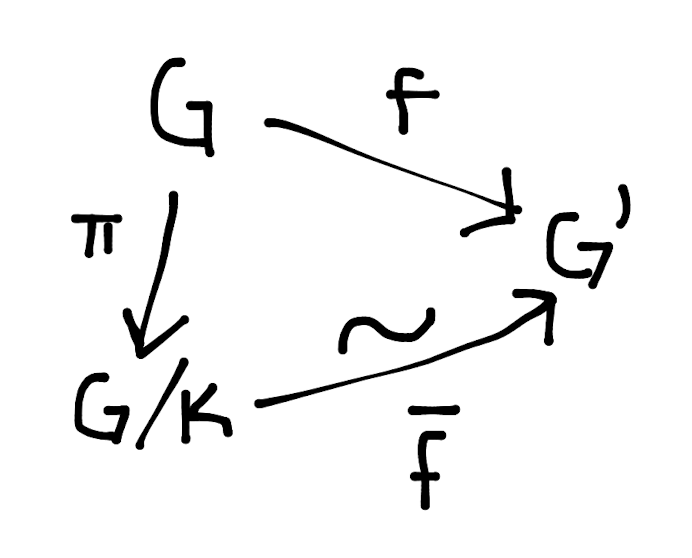
\includegraphics[width = 5cm]{images/lec6-2.png}

% https://tikzcd.yichuanshen.de/#N4Igdg9gJgpgziAXAbVABwnAlgFyxMJZARgBoAGAXVJADcBDAGwFcYkQBxAchAF9T0mXPkIpypYtTpNW7DgHoA0nwEgM2PASLiqNBizaJOfKTCgBzeEVAAzAE4QAtkjIgcEJOJAAjGGCieNIz0vowACkKaoiB2WOYAFjggejKGIAA66RC0MHaMWGAwwDa8KrYOzogATDTugdIG7DZlIPZOSDVuHoiu+rJGmWhYySDBoREaIuyxCUm8lLxAA
\begin{tikzcd}
G \arrow[r, "f"] \arrow[d, "\pi"'] & G' \\
G/K \arrow[ru, "\overline{f}"']    &   
\end{tikzcd}
\end{center}
commutes. 

So $f = \bar{f} \circ \pi.$ So up to isomorphism, our original group homomorphism is the same as our new one. This is not surprising, because there is a correspondence between cosets of the kernel and points in the image. All we are saying is that that bijection is compatible with the group structures on both sides. So $\bar{f}([xk]) = f(x).$ This is known as the \textbf{First Isomorphism Theorem.}

\newpage